\documentclass[letterpaper]{article}

%% Language and font encodings
\usepackage[english]{babel}

%\usepackage[utf8]{inputenc}
\usepackage[T1]{fontenc}
%\usepackage{indentfirst}

%% Sets page size and margins
\usepackage[letterpaper,top=1in,bottom=1in,left=1in,right=1in,margin=1in]{geometry}

%% Useful packages
\usepackage{etoolbox}
\usepackage{setspace}
\usepackage{subcaption}
\usepackage{float}
\usepackage{amsmath}
\usepackage{svrsymbols}
\usepackage{titletoc}
\usepackage[titles]{tocloft}
\usepackage{tikz-feynman}
\tikzfeynmanset{compat=1.1.0}

%%Quote configuration%%
\AtBeginEnvironment{quote}{\singlespacing\small}

%%Formatting Contents%%
\usepackage{titlesec}
\titleformat{\section}[block]{\color{black}\Large\bfseries\filcenter}{}{1em}{}
\renewcommand{\cftsecfont}{\color{black}\normalfont}
\renewcommand{\cftsecpagefont}{\color{black}\normalfont}
\newcommand*{\BeginNoToc}{%
 \addtocontents{toc}{%
   \edef\protect\SavedTocDepth{\protect\the\protect\value{tocdepth}}%
  }%
  \addtocontents{toc}{%
    \protect\setcounter{tocdepth}{-10}%
  }%
}
\newcommand*{\EndNoToc}{%
  \addtocontents{toc}{%
    \protect\setcounter{tocdepth}{\protect\SavedTocDepth}%
  }%
}

\addto\captionsenglish{
	\renewcommand{\contentsname}{\hfill \normalfont TABLE OF CONTENTS\hfill\vspace{1.5\baselineskip}}}
\addto\captionsenglish{
	\renewcommand{\listfigurename}{\hfill \normalfont LIST OF FIGURES\hfill\vspace{1.5\baselineskip}}}
\addto\captionsenglish{
	\renewcommand{\listtablename}{\hfill \normalfont LIST OF TABLES\hfill\vspace{1.5\baselineskip}}}
\usepackage{afterpage}

\DeclareRobustCommand*{\contheading}{%
  \afterpage{{\normalfont\Large\bfseries{\centering
       \normalfont TABLE OF CONTENTS (continued)\par\bigskip}}\vspace{1.5\baselineskip}
    {\normalfont\bfseries \normalfont Chapter \hspace{5.3in} \normalfont Page\vspace{1\baselineskip}
    }
  }
}

\DeclareRobustCommand*{\contfigures}{%
  \afterpage{{
      {\normalfont\Large\bfseries\centering
 \normalfont LIST OF FIGURES (continued)\par\bigskip}}\vspace{1.5\baselineskip}
      {\normalfont\bfseries{\hspace{-11mm} \normalfont Figure}\hfill \normalfont Page}\vspace{1.2\baselineskip}
  }
}
%%%%%%%%%%%%%%%%%%%%

%% Useful commands
\renewcommand{\cftdot}{}

%% Bibliography
\bibliographystyle{ieeetr}

%%%%%%%%%%%%%%%%%%%%%%%%%%%

  %%%%%%%%%%%%%%%%%%%%%%%%%%%%%%%%%%%%%%%%%%%%%%%%%%%%%%%%%%%%%%%%%%%%%%%%%%%%%%%%%%%%%%%%%%%%%%%%%%%
\begin{document}

%title page
\centering
\large{SECURE PRIVACY PRESERVING DEEP LEARNING AGAINST GAN ATTACKS}\\
[8\baselineskip]
\doublespace{
A Thesis by\\
Aseem Prashar\\
Master of Science, Wichita State University, 2020\\
Bachelor of Engineering, BITS-Pilani, 2013}\\
[6\baselineskip]
\singlespacing{
 Submitted to the Department of  Electrical Engineering and Computer Science\\
 and the faculty of the Graduate School of \\
 Wichita State University\\
 in partial fulfillment of\\
 the requirements for the degree of\\
  Master of Science} \\
[10\baselineskip]
May 2020
\pagenumbering{roman}
\thispagestyle{empty}
\pagebreak

%copy right page
\ 
\vspace{3in}
\begin{center}
\textcopyright\doublespacing{
Copyright 2020 by Aseem Prashar \\
All Rights Reserved}
\end{center}
\thispagestyle{empty}
\pagebreak

%signature title page
\begin{center}
SECURE PRIVACY PRESERVING DEEP LEARNING AGAINST GAN ATTACKS\\
[3\baselineskip]
The following faculty members have examined the final copy of this thesis for form and content, and recommend that it be accepted in partial fulfillment of the requirements for the degree of Master of Science with a major in Computer Science. \\
[4\baselineskip]
\raggedright{

\rule{3.75in}{0.4pt}\\
Sergio Salinas, Committee Chair} \\
[3\baselineskip]
\rule{3.75in}{0.4pt}\\

Akmal Mirsadikov, Committee Member \\
[3\baselineskip]

\rule{3.75in}{0.4pt}\\
Remi Chou, Committee Member \\
[3\baselineskip]

\rule{3.75in}{0.4pt}\\
Ajita Rattani, Committee Member \\
[3\baselineskip]

\end{center}
\pagebreak


%%%%%%%%%%%%%% DEDICATION %%%%%%%%%%%
\begin{center}
DEDICATION \\
\vspace*{2in}
I dedicate this thesis to my family, friends, and colleagues. 
\end{center}
\pagebreak

%%%%%%%%%%%%%%%%%%EPIGRAPH%%%%%%%%%%%%%%%%%%
\begin{center}
\vspace*{3in}
Somewhere, something incredible is waiting to be known. 
\end{center}
\pagebreak

%%%%%%%%%%ACKNOWLEDGEMENTS%%%%%%%%%%%%%%%%
\begin{center}
ACKNOWLEDGEMENTS\\
\end{center}
\vspace*{1\baselineskip}
\raggedright{
\setlength{\parindent}{0.50in}
\doublespacing{

I would like to thank my adviser, Sergio Salinas, for his thoughtful input, guidance and support in all stages of this project. I also extend my gratitude to members
of my committee, Ajita Rattani, Remi Chou and Akmal Mirsadikov for their valuable time and consideration. 

}
}
\pagebreak

%%%%%%%%%%%%%%%%%%%%%%%%ABSTRACT%%%%%%%%%%%%%%%
\begin{center}
ABSTRACT\\
\end{center}
\vspace*{1\baselineskip}
\raggedright{
\setlength{\parindent}{0.50in}
\doublespacing{


Deep learning is a class of machine learning algorithms that use a cascade of multiple layers of non-linear processing units for feature
extraction and transformation. Artificial neural network based
deep learning is becoming increasingly popular in a variety of fields. Deep learning benefits from larger input data sets and can be revolutionary to organizations that have access to sizeable raw data. In
the recent years, researchers have proposed decentralized collaborative learning architectures that allow multiple participants to share their data to train deep learning models. However, privacy and confidentiality concerns limit the application of this approach, preventing certain organizations such as medical institutions to fully benefit from collaborative deep
learning. 
To overcome this challenge, deep learning models that only share abstracted data for collaborative learning have recently been proposed. This approach helps users keep their actual datasets private whilst contributing to and befitting from collaborative learning. However, some researches have outlined threats that can use can take advantage of abstracted data to recreate original data and violate user privacy.

In this paper, we propose a collaborative deep learning approach that allows an organization improve their deep-learning model while preserving its privacy from such attacks. 

Specifically, we design our approach to protect organizational data against attacks that involve a malicious participant that can learn meaningful information from the abstracted dataset. Our proposed system protects the organization's privacy by limiting the exposure of private data from users to foreign entities. 

Our solution does not involve computationally expensive cryptographic processes and relies on limiting the exposure of private dataset of participants. 
Our approach is flexible and can be adapted to work with different neural network architectures. We demonstrate the efficacy of approach by calculating the resulting accuracy on benchmark datasets.

}
}
\pagebreak
\newcommand\Decide[1]{#1}


%-----------------------------------------------------------------------------------
%Preface
%-----------------------------------------------------------------------------------
%%%%%%%%%%%%%%%%%% Table of Contents%%%%%%%%%%%%%%%%%%%


\tableofcontents
\addtocontents{toc}{{\bfseries \normalfont Chapter\hfill \normalfont Page\bigskip\par}}
%\addtocontents{toc}{\contheading} %%% INCLUDE FOR MULTIPE TOC PAGES %%%%%
\pagebreak

%%%%%%%%%%%%%%%%% List of tables %%%%%%%%%%%%%%%%%%

\BeginNoToc
\listoftables
\addtocontents{lot}{{\bfseries \normalfont Table\hfill \normalfont Page\bigskip\par}}
\pagebreak

%%%%%%%%%%%%%%%%% List of Figures %%%%%%%%%%%%%%%%%%

\listoffigures
\addtocontents{lof}{{\bfseries \normalfont Figure\hfill \normalfont Page\bigskip\par}}
%\addtocontents{lof}{\contfigures} %%% INCLUDE FOR MULTIPE PAGES %%%%%
\pagebreak 
\EndNoToc

\begin{flushleft}
%%%%%%%%%%%%%%%%%

%%%%%%%%%%%%%%% List of Symbols %%%%%%%%%%%%%%%%%%
\makeatletter
\def\sectionsuffic{}
\def\subsectionsuffix{\quad}
\def\subsubsectionsuffix{\quad}
\def\paragraphsuffix{\quad}
\renewcommand\@seccntformat[1]{\csname the#1\endcsname\csname#1suffix\endcsname}
\renewcommand\thesection{\protect\Decide{\@arabic\c@section}}
\renewcommand\thesubsection{\@arabic\c@section.\@arabic\c@subsection}
\renewcommand\Decide[1]{}
\makeatother

\allowdisplaybreaks
\begin{center}
\Large\bf \normalfont LIST OF SYMBOLS\\
\end{center}
\begin{center}
\doublespacing{
\begin{align*}
&\nu &&\text{Neutrino}\\
&\gamma  &&\text{Photon/Gamma}\\
&\text{c}  &&\text{Speed of Light}
%make sure to have no space on your last line
\end{align*}
}
\end{center}

%%%%%%%%%%%%%%%%%%%%%%%% Begin Chapters %%%%%%%%%%%%%%%%%%%
%Introduction
\pagebreak
%-----------------------------------------------------------------------------------
\section*{CHAPTER I}
%-----------------------------------------------------------------------------------
\vspace{0.25in}
\section{INTRODUCTION}

\pagenumbering{arabic}
\setlength{\parindent}{0.50in}
\doublespacing{

In the past few decades, deep learning has generated a lot of interest in the research and academic community due to its great ability
to automatically classify large amounts of data. This has led to breakthroughs in many fields ranging
from autonomous driving, and natural language processing to genetic research \cite{young2018recent, al2017deep, huval2015empirical, danaee2017deep}.

%%%%%%%%%%% INSERT A FIGURE %%%%%%%%%%%%%%%
\begin{figure}[H]
  \centering
    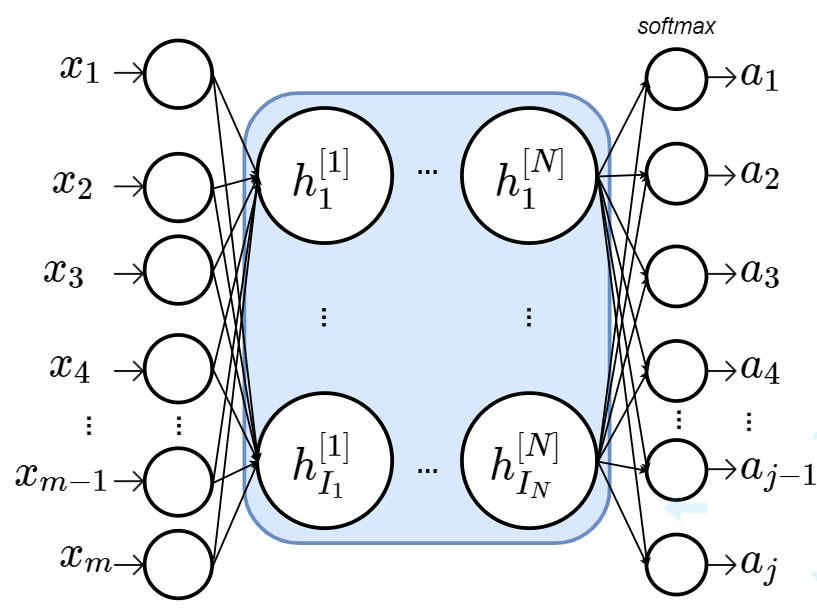
\includegraphics[width=3in]{SimpleNN.png}
    \caption[A simple neural network.]{\label{fig:atomsize} A neural network with $m$ inputs, $j$ outputs,  $N$  hidden layers, and $I$ neurons per layer.}
  \end{figure}
\addtocontents{lof}{\vspace{\normalbaselineskip}}


\pagebreak



%-----------------------------------------------------------------------------------
\section*{CHAPTER II}
%-----------------------------------------------------------------------------------


\vspace{0.25in}
\section{RELATED WORK}
\addtocontents{toc}{\vspace{\normalbaselineskip}}
Deep neural networks have outperformed traditional machine learning approaches for many tasks, and are the tool of choice in many
fields. Specifically, Deep learning has been successfully used for facial recognition \cite{krizhevsky2012imagenet, sun2014deep, ding2015robust}, image classification, 
\cite{simard2003best, ma2015hyperspectral, zhong2011bilinear}, and speech recognition \cite{hinton2012deep, graves2013speech, noda2015audio}, where it is expected to achieve better
performance than humans in the near future. However, directly applying these techniques in fields that deal with private data is
challenging. The reason is that they need to centrally collect data at a third-party which organizations may not trust
\cite{chicurel2000databasing}. This is particularly challenging in medical and financial applications where the privacy of the users is
governed by federal legislation and is protected by law. 

\pagebreak
%-----------------------------------------------------------------------------------
\section*{CHAPTER III}
%-----------------------------------------------------------------------------------
\vspace{0.25in}
\section{DEEP NEURAL NETWORK}
\addtocontents{toc}{\vspace{\normalbaselineskip}}
Deep neural networks are a type of machine learning that has recently shown high accuracy in data classification tasks. Traditional
machine learning requires manual feature selection, which can be time consuming and inaccurate. In contrast, deep learning
learns the most relevant features in the data on its own. In other words, the deep neural networks can be trained with raw data without
the burden of preprocessing it. Since deep neural networks have more hidden layers compared to traditional neural networks, their
accuracy is proportional to the amount of data used for training, i.e., the larger the training data set the more accurate that the
deep neural networks become. These advantages make deep neural networks a very effective technique to perform data classification
tasks. In this section, we describe the architecture of deep neural networks and their training methods. 



%-----------------------------------------------------------------------------------
\subsection{Architecture}\label{sec:MLP}
%-----------------------------------------------------------------------------------

In this work, we consider multilayer perception (MLP), which is one of the most common deep neural network architectures. An
MLP is formed by multiple layers where each layer consists of many nodes. Each node takes 
as input a weighted average of the previous layer's node outputs, and the output of an special node called the bias.  
The nodes use a non-linear activation function to the compute their output. Together, the weights used in the weighted average and
the biases from the special neurons are called the parameters of the deep neural network.


Figure \ref{fig:SimpleNN} shows the structure of a typical classification MLP with $m$ input nodes and $j$ outputs nodes. The neural network
has $N$ hidden layers and each layer has $I$ neurons. Intuitively, this MLP takes a data sample represented as a vector of length
$m$ on its input layer, and outputs the probability that it belongs to the $j$th category on the $j$th output neuron.


\begin{equation}
a^i_k=f(W_k a_{k-1})
\end{equation}
\noindent

\bigskip

%---------------------------------------------------------------------
\subsection{Training}
%---------------------------------------------------------------------
Before a neural network can be used to perform inference, e.g., classify images, it needs to be trained to learn the highly non-linear
relationships between the inputs and the correct outputs. Training finds the 
parameters of the deep neural network, i.e., its the weights and biases, that result in the inferences with the highest accuracy.


%---------------------------------------------------------------------
\subsubsection{Gradient Descent Algorithm}
%---------------------------------------------------------------------
The GD algorithm finds the parameter updates in two steps: error forward propagation and back propagation. 

%---------------------------------------------------------------------------------
\subsubsection{Stochastic Gradient Descent}
%---------------------------------------------------------------------------------

Although the GD algorithm is effective at finding the parameters of DNNs, all  training samples in the dataset need to be processed
before a single update is made to the parameters. That is, the algorithm processes the complete training data at each iteration. 
This is computationally intensive and time consuming. 

\pagebreak
%-----------------------------------------------------------------------------------
\section*{CHAPTER IV}
%-----------------------------------------------------------------------------------
\vspace{0.25in}
\section{PROBLEM FORMULATION}
\addtocontents{toc}{\vspace{\normalbaselineskip}}

In this section, we describe our considered collaborative deep learning model, and the threat model. 

%---------------------------------------------------------------------------------
\subsection{System Model} \label{sec:systemModel}
%---------------------------------------------------------------------------------
\begin{figure}[H]
  \centering
    \includegraphics[width=3in]{ClassificationNN.png}
    \caption[A simple neural network.]{\label{fig:ClassNN} Neural network depicting an image with $m \times m$ pixels fed as input, $j$ outputs  $N$  hidden layers and with $I$ neurons in layer.}
  \end{figure}
\addtocontents{lof}{\vspace{\normalbaselineskip}}



\begin{table}[ht]
\centering % used for centering table
\caption[Pym injection Trials]{Injection Trials} % title of Table
\label{table:pym} % is used to refer this table in the text
\begin{tabular}{*{15}{c}} % centered columns (4 columns)
\hline\hline %inserts double horizontal lines
Trial & Method & Result  \\ [0.5ex] % inserts table
%heading
\hline% inserts single horizontal line
1 & Hypodermic Injection & Dizziness \\ % inserting body of the table
2 & Oral Ingestion (2.46) & Vomiting \\
3 & Bio-injection suit  & Full size control  \\
\hline %inserts single line
\hline

\end{tabular}
\end{table}
\addtocontents{lot}{\vspace{\normalbaselineskip}}
%%%%%%%%%%%%%

\clearpage





























%-----------------------------------------------------------------------------------
\section*{CHAPTER III}
%-----------------------------------------------------------------------------------

\vspace{0.25in}
\section{CONCLUSION}
With the injection of pym particles I am able to enter the quantum realm and speak with insects. Future work will include exploration of of enlarging myself and developing crime fighting alter egos (see Appendix \ref{App:A}).

%%%%%%%%%%%%%%%%%%%%%%%%%%%%Bibliography%%%%%%%%%%%%%%%%%%%%%%%%%%%%%%
\newpage

\begin{center}
\vspace*{\fill}
\addcontentsline{toc}{section}{BIBLIOGRAPHY}
\section*{\normalfont BIBLIOGRAPHY}
\vspace*{\fill}
\end{center}
\newpage
\let\oldaddcontentsline\addcontentsline% Store \addcontentsline
\renewcommand{\addcontentsline}[3]{}% Remove functionality of \addcontentsline
\renewcommand\bibname{\normalfont BIBLIOGRAPHY}
\bibliography{sample}
\let\addcontentsline\oldaddcontentsline% Restore \addcontentsline

%%%%%%%%%%%%%%%%%%%%%%%%%%%%Appendix%%%%%%%%%%%%%%%%%%%%%%%%%%%%%%%%
\newpage
\appendix
\addcontentsline{toc}{section}{APPENDIXES}
\addtocontents{toc}{\vspace{\normalbaselineskip}}
\renewcommand\thesubsection{\Alph{subsection}}
\newpage

\begin{center}
\vspace*{\fill}
\section*{\normalfont APPENDIXES}
\vspace*{\fill}
\end{center}

%%%%%%%%%%%%%%%%% Appendix A %%%%%%%%%%%%%%%%%%%%%%%
\newpage
\section*{\normalfont APPENDIX A} \label{App:A}
\section*{Possible Alter Egos} 
\addcontentsline{toc}{subsection}{A. Possible Alter Egos}
\addtocontents{toc}{\vspace{\normalbaselineskip}}
Possible alter egos to facilitate crime fighting: Ant-Man, Giant Man, Quantum-Man, The Wasp, The Whisper. 

%%%%%%%%%%%%%%%%% Appendix B %%%%%%%%%%%%%%%%%%%%%%%
\newpage
\section*{\normalfont APPENDIX B} \label{App:B}
\section*{My Awesome Suit} 
\addcontentsline{toc}{subsection}{B. My Awesome Suit}
\addtocontents{toc}{\vspace{\normalbaselineskip}}

Here's a look at my awesome suit. 

}

\end{flushleft}
\end{document}
